\section{Writing a GUI for Your Application}
\label{sec:gui}

\subsection{Application Framework}
A GUI can help users effectively use an
application.  Application GUI's have many levels, from simple and straight
forward, to complex and time consuming to write.  Many books have been written
about GUI
programming, for a good overall introduction to GUI programming please look at
Cooper's book, \textbf{"About Face: the Essentials of User Intergace Design,
IDG Books World Wide, 1995"}. For for look and feel issues, refer to the Motif
style guide, \textbf{"OSF/Motif Style Guide, Revision 1.2, Prentice Hall, 1993?"}. 
Several of us in the AIPS++ group use
Welch's book, \textbf{"Practicle Programming in Tcl and Tk, Prentice Hall, 1995"},
about TCL/TK programming for nuts and bolts of 
GUI programming.

Glish/Tk uses much of Tcl/Tk philosophy so books
about Tcl/Tk programming may provide some insight.  Unfortunately Glish/Tk
doesn't have all the functionality of Tcl/Tk, so if you need a feature and
it isn't currently supported ask.
\subsubsection{Philosophy}
All AIPS++ applications that have a GUI should present a similar look
and feel to the user.  A "similar look and feel" means:
\begin{enumerate}
\item Provide a consistent menubar.  A typical menubar consists of File, Options, and Help menus.  Other traditional menus include Edit and View.  Other 
application specific menus may be added.
\item Use a consistent naming/action convention for buttons.  The standard 
button labels are:
\begin{itemize}
\item OK, do the requested action, dismiss the window;
\item Apply, do the requested action but don't dismiss the window;
\item Reset, reset all the values in the window to thier previous values,
don't dismiss the window; and
\item Cancel, dismiss the window and do nothing.
\end{itemize}
If it's clear to the user use it, in our
printer example rather
than labeling a button OK, it makes more sense to use the label Print.
\item Call the same file/data chooser window, so the user is not confronted
with a customized load/save window for every application.
\item Use the same message window layout to display informational content.  
Message windows are either blocking, program waits for a user response, or non-blocking, program continues.  Choose to block only when user input is necessary
for continued program execution.
\item Message windows which require the user to choose one of several options
should block the application until the user has made a choice.
\item Provide an informational title for every window.
\item Use either a progress bar or a status message at the footer of the window
to let the user know something is going on, or happened.
\end{enumerate}
Figure~1 shows the major parts of a command action window.  Please try and
follow the motif style guide when assembling the parts in the "work area".
\begin{figure}[here]
\epsfig{file=aips2gui.eps}
\caption{The basic AIPS++ gui window.}
\end{figure}
There are several standard utilities/building blocks for constructing a 
consistent interface,  
\begin{itemize}
\item \htmlref{guiframework}{guiutils:guiframework},
\item \htmlref{filechooser}{guiutils:},
\item \htmlref{datachooser}{guiutils:},
\item \htmlref{choices}{guiutils:}, and
\item miscellaneous functions found in \htmlref{guiutils}{guiutils:}.
\end{itemize}
Please use them rather than rolling your own.

If you're
doing a simple load and go interface we hope to provide a "load-and-go utility"
that will let you specify a few glish records and the produce a standard GUI.
\subsubsection{An example}

The example comes from \htmladdnormallink{printer.g}{../../../code/trial/implement/Tasking/printer.g}. 
It illustrates setting up a help menu and action buttons for
the printer objects gui.  The event handler self.printfunction follows the
code snippet (it preceedes it in the actual code).

\begin{verbatim}

    public.gui := function(files="", remove=F, landscape=F)
    {
        wider self
        files := as_string(files)
        self.files := files
        self.remove := remove
 
        if (landscape) {
            self.mode := 'l'
        }
 
        if (!have_gui()) {
          self.logger.log('', 
           'SEVERE', 'Does not appear to be connected to a windowing system',
                          'printer::gui')
            fail 'Does not appear to be connected to a windowing system'
        }
\end{verbatim}

This code initializes some "self" variables and checks if the
user is running in a windowing system, if not it the function exits with a
fail.  If you write gui functions, you should check whether a user is capable
of running your function.

\begin{verbatim}
        # set the help menu
        helpmenu := [=];
        helpmenu::text := 'Help';
        helpmenu.print := [=];
        helpmenu.print.text := 'Printing';
        helpmenu.print.action := function(){help('Refman:utility.printer')};
        helpmenu.reference := [=];
        helpmenu.reference.text := 'Reference';
        helpmenu.reference.action := function(){help('Refman')};
        helpmenu.about := [=];
        helpmenu.about.text := 'About AIPS++...';
        helpmenu.about.action := about;
 
        # set the action buttons
        actions := [=];
        actions.print := [=];
        actions.print.text := 'Print';
        actions.dismiss := [=];
        actions.dismiss.text := 'Dismiss';
 
        # application's window
        self.gf      := guiframework('AIPS++ Printer control', F, helpmenu,
                                      actions)
 
        # add the handlers
        self.gf.addactionhandler('dismiss', self.gf.dismiss)
        self.gf.addactionhandler('print', self.printfunction);

\end{verbatim}
This section of code, sets up the help menu, action buttons, creates the
frame work and adds the action handlers. It's important that the action 
handlers be defined before you add them, otherwise you handler will not be
called.

\begin{verbatim}

        # Get the workframe and do everything else the same.
        self.wholeframe := self.gf.getworkframe()
 
        #
        self.filesframe      := frame(self.wholeframe, side='left')
        self.fileslabel      := label(self.filesframe, 'Files:',width=20)
        self.filesentry      := entry(self.filesframe)
        if (length(files) > 0) {
           send self.filesentry->insert(files)
           send self.filesentry->disabled(T)
        } else {
           whenever self.filesentry->return do {
             self.files := $value
           }
        }
 
        # Remove
        self.removeframe     := frame(self.wholeframe, side='left')
        self.removelabel     := label(self.removeframe,
                                 'Remove after printing:',width=20)
        self.removebutton    := button(self.removeframe, 'Yes',
                                       type='check')
 
        send self.removebutton->state(self.remove)
        whenever self.removebutton->press do {
          self.remove := request $agent->state()
        }
 
        ... Lots of stuff removed ...

        return T
    }

\end{verbatim}
After grabbing the work area frame, we go about the job of adding frames, 
buttons and labels to the frame work.

\begin{verbatim}
    self.printfunction := function(){
           wider self; 
           wider public;
           self.files := request self.filesentry->get()
           self.printer_name := request self.printerentry->get()
           if (length(self.files) == 0 ||
              (length(self.files)==1 && self.files[1] == '')) {
              self.logger.note('Not printing any files',
                                origin='printer::gui')
              a := infowindow('No files to print', 'AIPS++ Printer Control');
            } else {
              public.print(self.files, self.remove)
              self.gf.dismiss();
           }
        }
\end{verbatim}

Here's the call back used to print the file(s). The call back need
not be a "self" function.  An alternative form would be:

\begin{verbatim}
        self.gf.addactionhandler('print', function(){
           wider self; 
           wider public;
           self.files := request self.filesentry->get()
           self.printer_name := request self.printerentry->get()
           if (length(self.files) == 0 ||
              (length(self.files)==1 && self.files[1] == '')) {
              self.logger.note('Not printing any files',
                                origin='printer::gui')
              a := infowindow('No files to print', 'AIPS++ Printer Control');
            } else {
              public.print(self.files, self.remove)
              self.gf.dismiss();
           }
        });
\end{verbatim}

How you add the callbacks is a matter of style.  For complicated functions
it is better to define your functions first
rather than define them in the argument to addactionhandler. For short
functions, a few lines, in-lining the function call works just as well.

\subsection{Input Forms}
For the programmer who want's a GUI but doesn't need the fine control of GUI 
components offered by glishTk, we have two stylized input forms available.
The programmer specifies a \textit{Screen Input Record} and invokes either a
\texttt{gui.inputform} or \texttt{gui.tabform}.  The following three examples
are from inputframe.g.  The first example builds a stand-alone form, the second
uses a parent frame, and the third shows a pseudo-tab form.

The \textit{Screen Input Record} is defined as\\
\begin{tabular}{ll}
title & text in the window title\\
label & text in the window\\
actions & (a.label a.function)record of functions\\
layout & ignored for now\\
data & record of datums\\
progress & T or F (Shows a progress bar, not implemented)\\
\end{tabular}
\\\\Each member of a \textit{data record} is an \textit{input-field}  and has
the following members\\\\
\begin{tabular}{ll}
label & Description of datum field\\
type & one of the following: string, float, double\\
     & long, integer, file, table, time, date, or\\
     & text - string with more than oneline of text\\
required & boolean, T if required for processing\\
hint & one of: check, radio, list, menu\\
enums & vector of allowed values\\
multiple & boolean for allowing multiple choices of enums\\
range.min & minimum value\\
range.max & maximum value\\
default & default value\\
verify & function to verify input\\
mask & display mask (not implemented)\\
help.url & a URL to drive a web browser (not implemented)\\
help.text & text for help of this field (not implemented)\\
\end{tabular}

If the type is file or table, a file or data-chooser is launched. 

If the type is an integer with a range of values then it will appear as a
slider. 

If there are more than four enums, a list box will be used otherwise check
or radio buttons will be used.  Hints will be honored, so you may have more
than four check or radio buttons by specifying the hint record.

In the first example(output form shown in Figure~2), the programmer supplies the parent frame gui.inputform
Each of the controls are illustrated.
\begin{figure}[here]
\epsfig{file=guiinputframe.ps, height=5in}
\caption{An example of the AIPS++ Input Form window.}
\end{figure}

\begin{verbatim}
gui.testframe := function()
{  global gui;
#
   wreck := [=];
   wreck.actions := [=];  
   wreck.data := [=];  
#
   wreck.title := 'Test of input form';
#
   wreck.data.name := [=];
   wreck.data.name.label := 'Name';
   wreck.data.name.type := 'string';
   wreck.data.name.default := 'Your name here'
#
   wreck.data.slider := [=];
   wreck.data.slider.label := 'Slider';
   wreck.data.slider.type := 'int';
   wreck.data.slider.range.min := 1;
   wreck.data.slider.range.max := 100;
   wreck.data.slider.default := 42;
#
   wreck.data.rb := [=];
   wreck.data.rb.label := 'radio button';
   wreck.data.rb.type := 'string';
   wreck.data.rb.default := "three"
   wreck.data.rb.enums := "one two three four";
#
   wreck.data.cb := [=];
   wreck.data.cb.label := 'check button';
   wreck.data.cb.hint := 'check';
   wreck.data.cb.type := 'string';
   wreck.data.cb.default := "one three"
   wreck.data.cb.enums := "one two three four";
#
   wreck.data.lb := [=];
   wreck.data.lb.label := 'list box';
   wreck.data.lb.type := 'string';
   wreck.data.lb.multiple := F;
   wreck.data.lb.enums := "one two three four five six seven";
   wreck.data.lb.default := "five";
#
   wreck.data.file := [=];
   wreck.data.file.label := 'file';
   wreck.data.file.type := 'file';

 #
   wreck.data.data := [=];
   wreck.data.data.label := 'data';
   wreck.data.data.type := 'table';
#
   wreck.data.date := [=];
   wreck.data.date.label := 'date';
   wreck.data.date.type := 'date';
#
   wreck.data.time := [=];
   wreck.data.time.label := 'time';
   wreck.data.time.type := 'time';
#
   wreck.actions.go := [=];
   wreck.actions.go.label := 'Go';
   wreck.actions.go.function := function(data){print data;}
#
   wreck.actions.dismiss := [=];
   wreck.actions.dismiss.text := 'Dismiss';
#
   hmenu := [=];
   hmenu::text := 'Help';
   hmenu.about := [=];
   hmenu.about.text := 'About';
   hmenu.about.relief := 'flat';
   hmenu.about.action := about;
 
   gf := guiframework('Test for guiinputs', F, hmenu, F)
   fgf := gui.inputform(wreck, parent=gf.getworkframe());
   fgf.addactionhandler('dismiss', gf.dismiss);
}
\end{verbatim}

The second example is nearly identical to the first except that gui.inputform
creates the parent window and default help menu.

\begin{verbatim}
gui.testinputs := function()
{  global gui;
   
#
   wreck := [=];
   wreck.actions := [=];  
   wreck.data := [=];  
#
   wreck.title := 'Test of input form';
#
   wreck.data.name := [=];
   wreck.data.name.label := 'Name';
   wreck.data.name.type := 'string';
   wreck.data.name.default := 'Your name here'
#
...lots of lines deleted for brevity (all similar to gui.testframe)...
#
   wreck.actions.go := [=];
   wreck.actions.go.label := 'Go';
   wreck.actions.go.function := function(data){print data;}
#
   fgf := gui.inputform(wreck);
}
\end{verbatim}

The third example, Figure~3, shows a \textit{tab-input form}.  \textit{Tab-input forms} 
are most useful when you have an object with several methods.
\begin{figure}[here]
\epsfig{file=guitabframe.ps, width=\linewidth }
\caption{An example of the AIPS++ Tab-Input Form window.}
\end{figure}
\begin{verbatim}
gui.testtab := function()
{  global gui;
#
   wreck := [=];
 
   wreck1 := [=];
   wreck2 := [=];
   wreck3 := [=];
   wreck4 := [=];
   wreck5 := [=];
   wreck6 := [=];
 
   wreck1.actions := [=];  
   wreck1.data := [=];  
   wreck1.title := 'Test of tab form, pane 1';
#
   wreck2.actions := [=];  
   wreck2.data := [=];  
   wreck2.title := 'Test of tab form, pane 2';
#
   wreck3.actions := [=];  
   wreck3.data := [=];  
   wreck3.title := 'Test of tab form, pane 3';
#
   wreck4.actions := [=];  
   wreck4.data := [=];  
   wreck4.title := 'Test of tab form, pane 4';
#
   wreck5.actions := [=];  
   wreck5.data := [=];  
   wreck5.title := 'Test of tab form, pane 5';
#
   wreck6.actions := [=];  
   wreck6.data := [=];  
   wreck6.title := 'Test of tab form, pane 6';
#
   wreck1.data.name := [=];
   wreck1.data.name.label := 'Name';
   wreck1.data.name.type := 'string';
   wreck1.data.name.default := 'Your name here'
#
   wreck2.data.slider := [=];
   wreck2.data.slider.label := 'Slider';
   wreck2.data.slider.type := 'int';
 
   wreck2.data.slider.range.min := 1;
   wreck2.data.slider.range.max := 100;
   wreck2.data.slider.default := 42;
#
   wreck3.data.rb := [=];
   wreck3.data.rb.label := 'radio button';
   wreck3.data.rb.type := 'string';
   wreck3.data.rb.default := "three"
   wreck3.data.rb.enums := "one two three four";
#
   wreck4.data.cb := [=];
   wreck4.data.cb.label := 'check button';
   wreck4.data.cb.hint := 'check';
   wreck4.data.cb.type := 'string';
   wreck4.data.cb.default := "one three"
   wreck4.data.cb.enums := "one two three four";
#
   wreck5.data.lb := [=];
   wreck5.data.lb.label := 'list box';
   wreck5.data.lb.type := 'string';
   wreck5.data.lb.multiple := F;
   wreck5.data.lb.enums := "one two three four five six seven";
   wreck5.data.lb.default := "five";
#
   wreck6.data.file := [=];
   wreck6.data.file.label := 'file';
   wreck6.data.file.type := 'file';
#
   wreck1.data.data := [=];
   wreck1.data.data.label := 'data';
   wreck1.data.data.type := 'table';
#
   wreck2.data.date := [=];
   wreck2.data.date.label := 'date';
   wreck2.data.date.type := 'date';
#
   wreck3.data.time := [=];
   wreck3.data.time.label := 'time';
   wreck3.data.time.type := 'time';
#
   wreck1.actions.go := [=];
   wreck1.actions.go.label := 'Go';
   wreck1.actions.go.function := function(data){print data;}
#
   wreck1.actions.dismiss := [=];
   wreck1.actions.dismiss.text := 'Dismiss';
#
   wreck2.actions.go := [=];
   wreck2.actions.go.label := 'Go';
   wreck2.actions.go.function := function(data){print data;}
#
   wreck2.actions.dismiss := [=];
   wreck2.actions.dismiss.text := 'Dismiss';
#
   wreck3.actions.go := [=];
   wreck3.actions.go.label := 'Go';
   wreck3.actions.go.function := function(data){print data;}
#
   wreck3.actions.dismiss := [=];
   wreck3.actions.dismiss.text := 'Dismiss';
#
   wreck4.actions.go := [=];
   wreck4.actions.go.label := 'Go';
   wreck4.actions.go.function := function(data){print data;}
#
   wreck4.actions.dismiss := [=];
   wreck4.actions.dismiss.text := 'Dismiss';
#
   wreck5.actions.go := [=];
   wreck5.actions.go.label := 'Go';
   wreck5.actions.go.function := function(data){print data;}
#
   wreck5.actions.dismiss := [=];
   wreck5.actions.dismiss.text := 'Dismiss';
#
   wreck6.actions.go := [=];
   wreck6.actions.go.label := 'Go';
   wreck6.actions.go.function := function(data){print data;}
#
   wreck6.actions.dismiss := [=];
   wreck6.actions.dismiss.text := 'Dismiss';
#
   wreck.tab1 := wreck1;
   wreck.tab2 := wreck2;
   wreck.tab3 := wreck3;
   wreck.tab4 := wreck4;
   wreck.tab5 := wreck5;
   wreck.tab6 := wreck6;
#   wreck::disallow := "tab3 tab4";
#   wreck::show := "tab3";
   wreck::categories := [=];
   wreck::categories.All := T;
   wreck::categories.First3 := "tab1 tab2 tab3";
   wreck::categories.Last3 := "tab4 tab5 tab6";
   wreck::categories.Last3::label := 'Label for last 3 functions'
 
   fgf := gui.tabform(wreck, tabcount=3, side='left');
   fgf.dismisshandler('dismiss')
}
\end{verbatim}
